\documentclass[thesis.tex]{subfiles}
\begin{document}
\chapter{Apps and App Stores}
\label{chap:apps-and-stores}

\section{App Stores}

App stores are the primary mechanism for distributing software on smart phones.
Whilst iOS is limited to just one store (Apple's App store), the Android ecosystem is more diverse with multiple stores available for multiple different purposes.
The dominant app store on Android is Google Play. 
Unlike iOS, Google isn't the sole app vendor however.
Some device vendors add their own stores to their devices as a feature.
Amazon, for example, do this with their Kindle Fire tablets, where Kindle owners can download discounted apps.
Some vendors, such as Samsung, add their own store this to highlight apps that use features specific to their phones (KNOX in Samsung's case).
In some regions (most notably China), using Google products can be problematic and local app stores are offered instead (such as QiHoo360, and Yandex).

For a manufacturer to install Google's store they must
comply with the Android \ac{CDD}~\cite{???}.  The \ac{CDD} describes how the
Android operating system should be configured and what features a device must
have to run Android.  If a manufacturer cannot pass the \ac{CTS} that tests
conformance with the \ac{CDD} then they cannot install the Play Store.

For manufacturers like \emph{Jolla} whose devices do not run
Android\footnote{They run Sailfish, which is based off of the Linux Foundation's
Mer operating system.}, but can emulate some parts of the Dalvik virtual machine
enough to run Android apps, third party stores like Yandex and Aptoide allow the
device to still benefit from apps designed for the Android ecosystem.

Precise numbers of apps in different stores is hard to obtain, but rough numbers for some of the largest stores are reported occasionally~(\autoref{fig:app-store-apps}).
Google and Apple's stores have (as of the end of 2016) around 2.5 million apps, with Amazon's store having considerably less.

\begin{figure}
  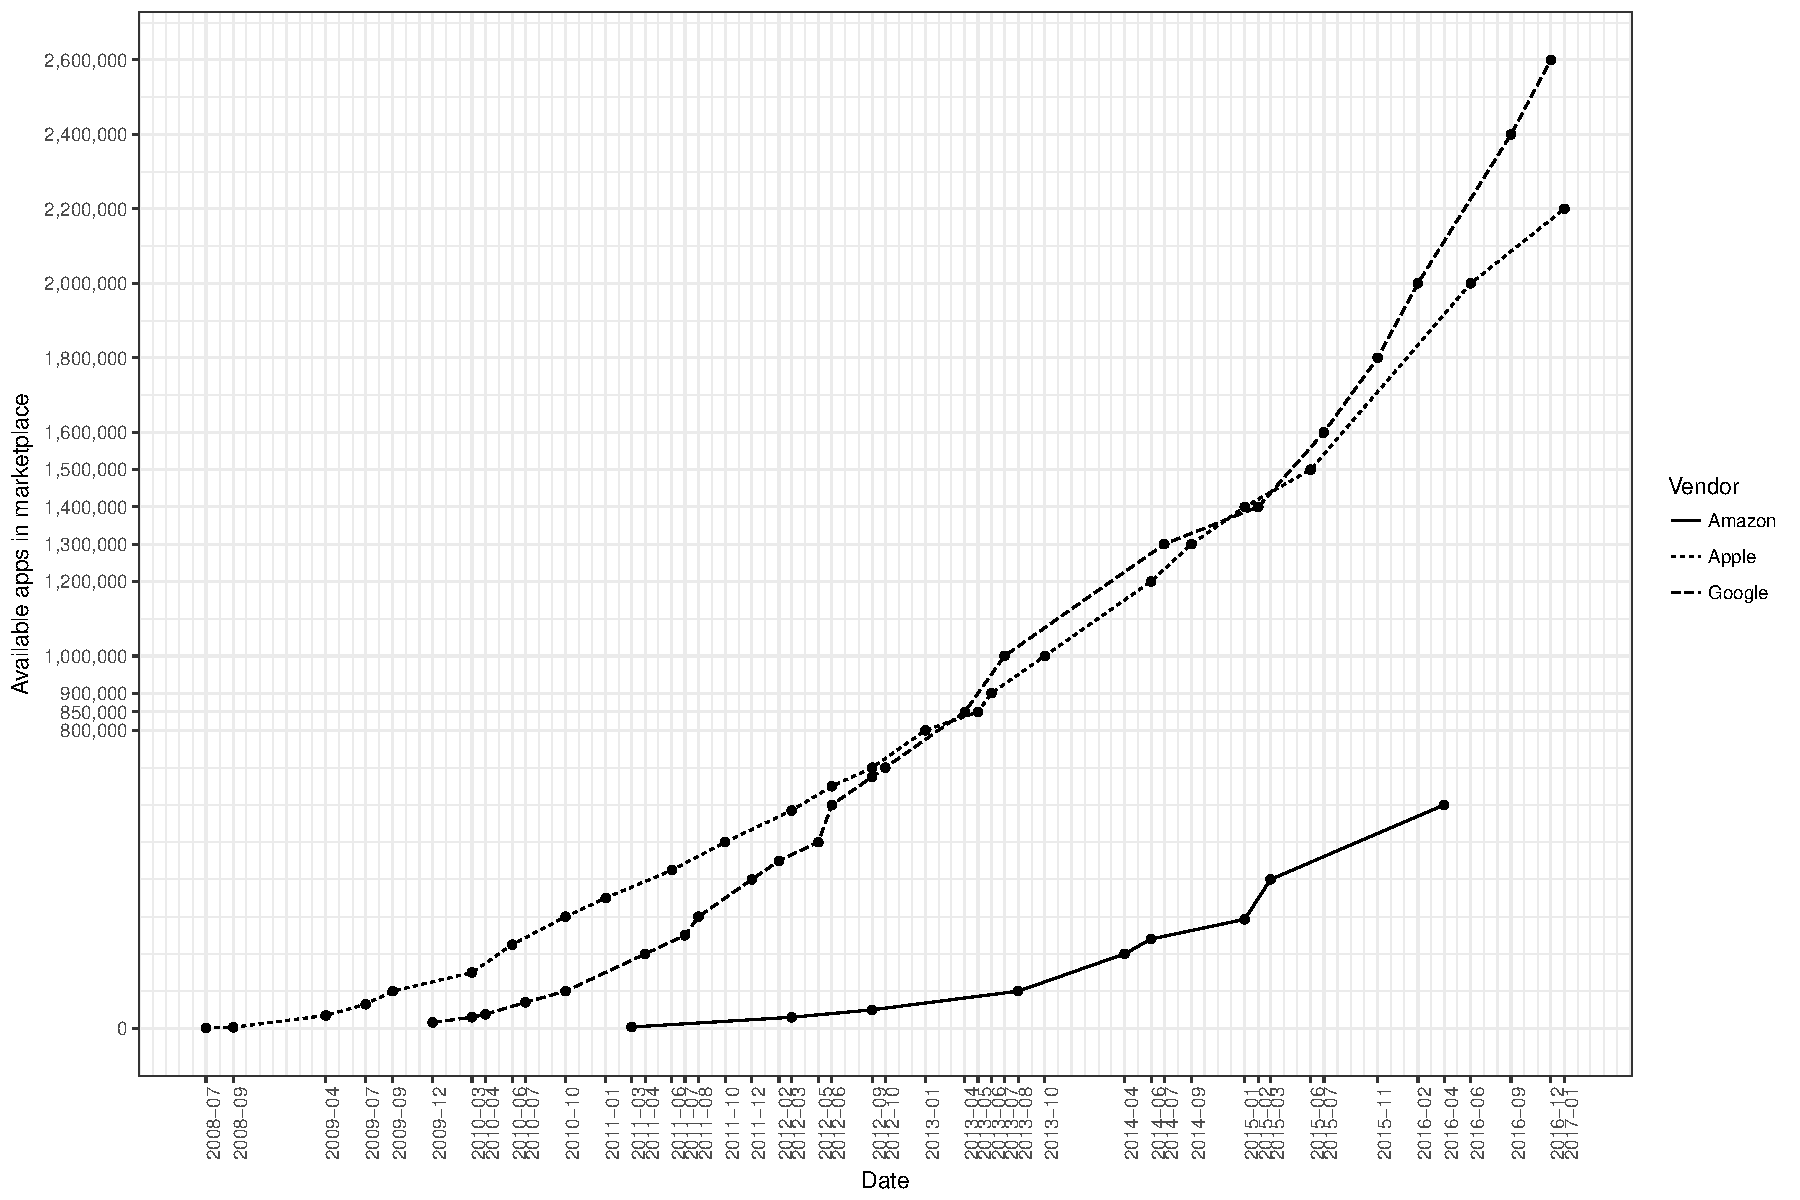
\includegraphics[width=\textwidth]{figures/app-store-apps.pdf}
  \caption[Reported numbers of different apps on various App marketplaces.]{%
    Reported numbers of different apps on various App marketplaces. Data taken from~\cite{statista_google_nodate,statista_apple_nodate,statista_amazon_nodate}.}
  \label{fig:app-store-apps}
\end{figure}

In this section we will focus on five different app stores: Apple's App Store,
Amazon's app store, Aptoide, Google Play and Yandex.  Apple's App Store is for iOS,
but the rest are for Android operating systems.  
Amazon's app store was opened in 2011 and was the primary app store for Amazon's
Kindle tablets released later that year.  Like Apple and Google's stores it is a
store controlled by a device manufacturer.

Yandex is a store primarily aimed at
the Russian and eastern European markets and it features a large number of
Russian language apps.  Some manufacturers, such as Nokia, installed Yandex over
Google's app store on devices sold in Russia. 




\paragraph{The other iOS stores}
\todo{Move to background?}

Apple's devices are limited normally only have access to Apple's App Store; however there is a second, unofficial, method of installing apps.
Jay Freeman's \emph{Cydia} is an alternative method for installing apps on jailbroken devices.
When a jailbreak is released they usually install the Cydia store as well.
Cydia itself is build atop of Debian's \emph{dpkg} framework and relies on various \emph{repositories} for hosting and distributing the apps.

Anyone is free to host their own repository but often the de facto \emph{``official''} repository is \emph{BigBoss}.
BigBoss is further split into three stores: free, CydiaStore with purchases handled by the Cydia store, and CydiaStore with purchases handled by the app and their own payment mechanisms.  To host an app in their store they list the following conditions~\cite{bigboss_host_2014}.

\begin{quotation}
  \begin{enumerate}
    \item You must own the app and be the developer of the content

    \item No porn or adult apps. No swagbucks style apps where user makes you money by shopping with your ID.

    \item You can only use one Cydia repository. If you submit here do not submit this to another major host elsewhere or it will have to be removed from one of the repositories. (You can host this in your own, private repository still just not any other major community source). There is no benefit to having duplicate packages in major sources as you get the same exposure by using just one.

    \item Screenshots for any GUI app are required. If you don’t provide screenshots, your submission will be delayed.

    \item Make sure your app is signed with ldid and properly built. We recommend you build with Theos but you can use whatever you want as long as you test in a jailbroken iOS enviornment. Thie means you should not be submitting xcode generated IPA files as this is a dead giveaway that you did not test properly.
  \end{enumerate}
\end{quotation}

The Cydia based stores are considerably less formal than the Android marketplaces, and they require less information and have less terms.
In part this may be because they are unofficial, and rely upon a jailbreak to be installed.  They are not backed by companies but instead are hosted and maintained by the jailbreaking community.  In this thesis we are not going to consider these stores as they are, by necessity, outside of the scope of the standard mobile ecosystems.  They are, howeverworth mentioning for the sake of completeness.

The other iOS stores worth mentioning (though again we will not consider them) are the piracy stores.
These exist to allow users to download pirated paid apps from the App Store for free.
Perhaps the most notable of these was the \emph{Installous} Cydia repo which hosted pirated apps for many years.
These stores come and go as they are shutdown; some working through Cydia, and some offering the pirated \emph{IPA} (Apple's app package format) for installation through iTunes.
Again, we will not cover these stores (in part because they are so transient) but they are worth mentioning.

\subsection{Exploring differences in terms between markets}.

With the various different app stores available, a user or developer might be interested in the differences between them.
Different stores require different amounts of identification from their users to buy and sell apps, or offer different terms and conditions.

Some stores may modify apps sold in them.  For Android users this can be particularly important as it changes the trust relationships around who can provide updates and who developed the app.

The precise terms for using these stores are hidden in user and developer agreements.
These hide within pages of legalese what the stores are \emph{contractually} allowed to do with a user's data and a developer's app.
To explore the differences we took user and developer from five different markets: Google Play, Amazon App Store, Apple's App Store, Yandex and Aptoide.
These five were chosen as they represent the biggest app marketplaces (Apple and Google Play) as well as some of the larger third party market places (Amazon and Yandex).
Yandex and Aptoide are market places that are often installed on Android devices that do not meet Google's criteria for the Play Store.

These five seem to cover many of the different use cases and terms for a store, though unfortunately they do not include a Chinese store.
The Chinese Android app markets are interesting as, unlike the rest of the world, they have grown without ever being in competition with Google's store.
Many of the apps featured on the front page of the \emph{Baidu} marketplace (China's largest), are unfamiliar, with only the games having recognisable icons (\autoref{fig:storefronts}).
Apps like WhatsApp Facebook and Candy Crush, that are featured on nearly every other app market are absent.
Unfortunately for a non-Chinese speaker the markets can be impenetrable, making finding and comparing terms of use difficult to impossible.
Future work should explore these markets further as they represent an important part of the mobile ecosystem largely unexamined by this dissertation.

\begin{figure}\centering
  \begin{minipage}{\linewidth}
    \begin{minipage}{0.48\linewidth}
      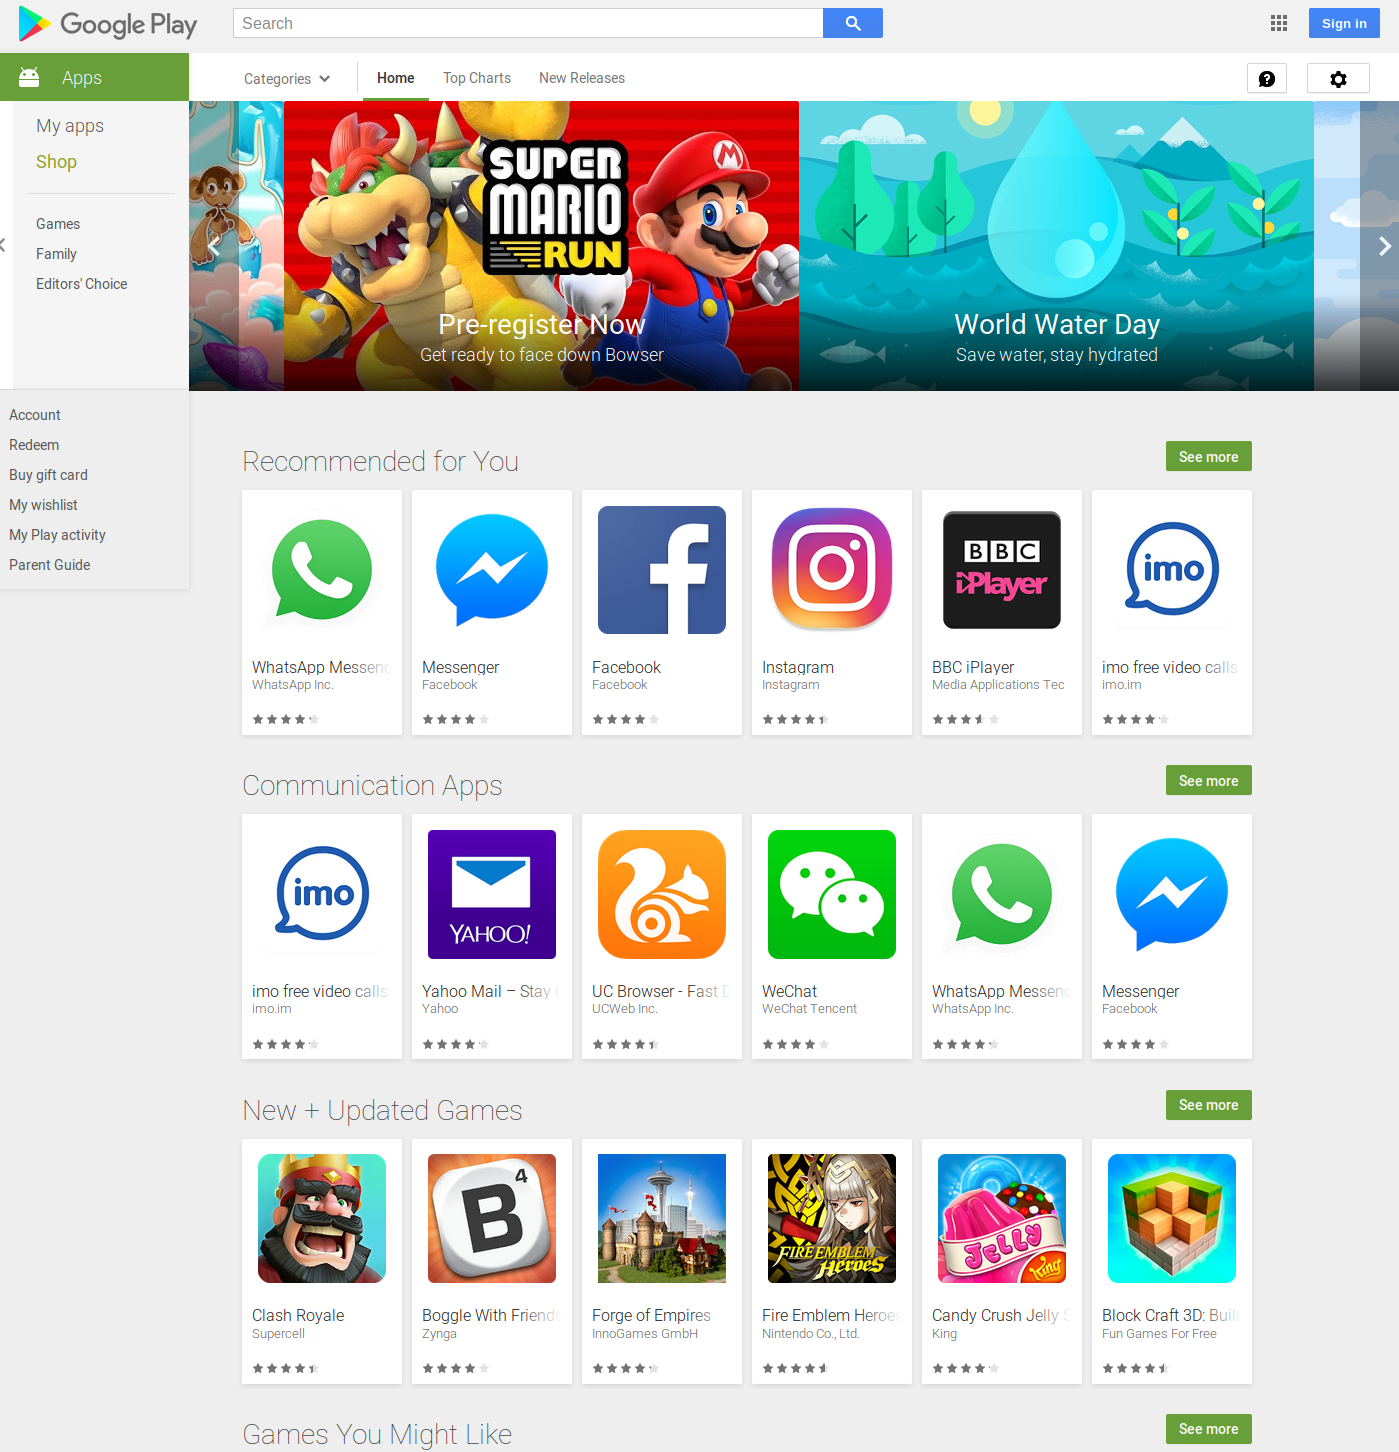
\includegraphics[width=\linewidth]{figures/google-storefront.png}
    \end{minipage}
    \begin{minipage}{0.48\linewidth}
      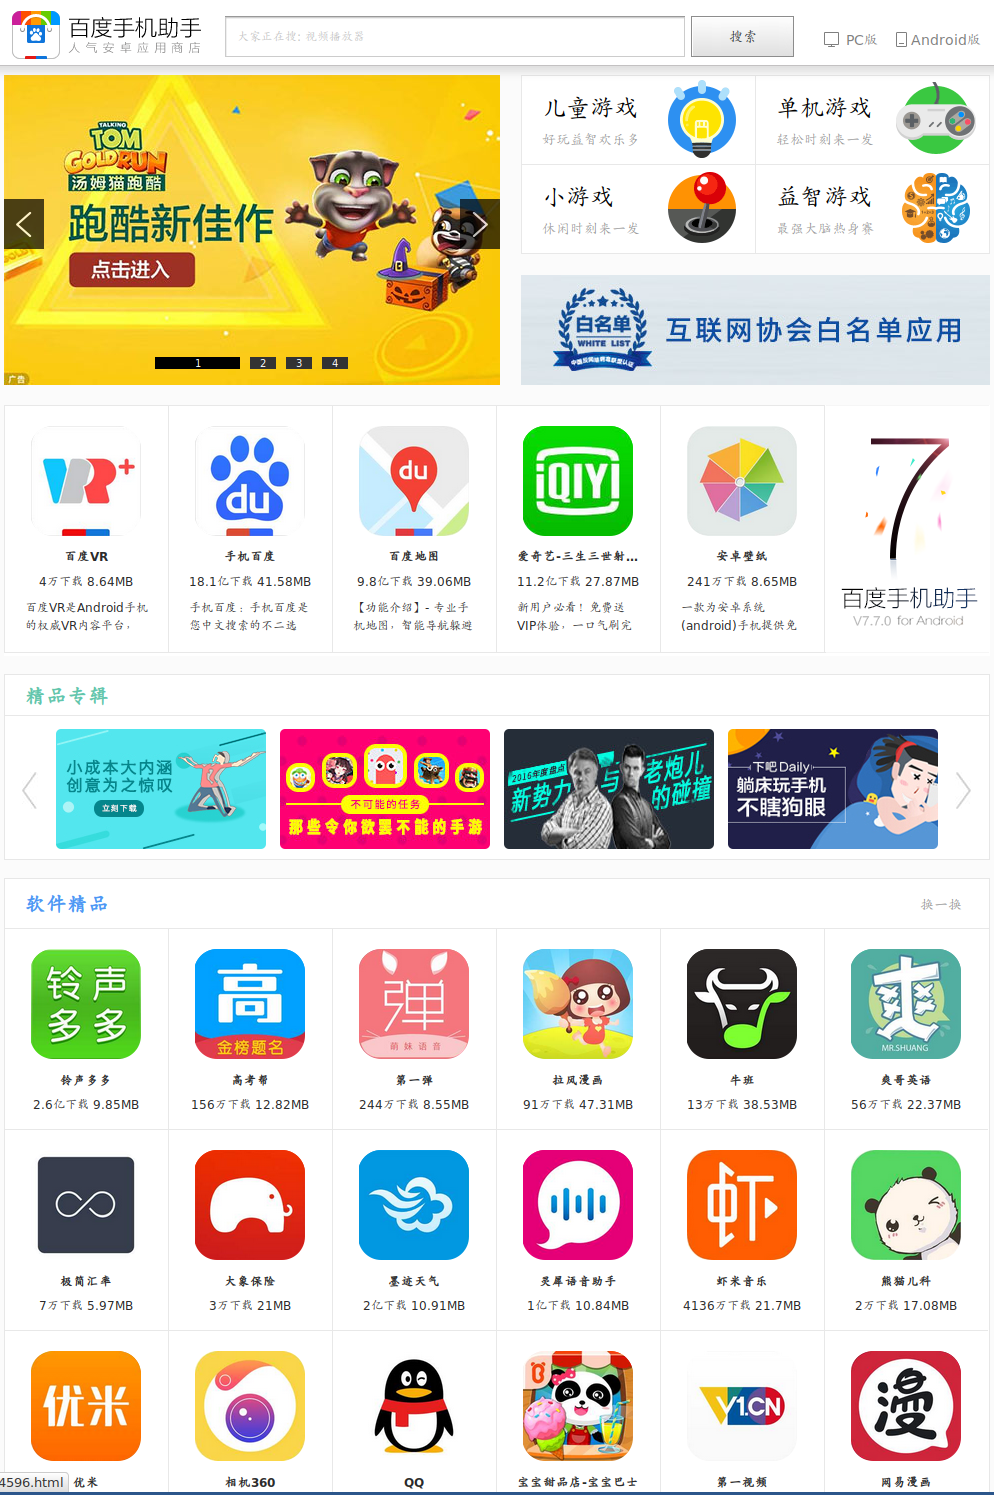
\includegraphics[width=\linewidth]{figures/baidu-storefront.png}
    \end{minipage}
  \end{minipage}
  \caption{Different storefronts for Google Play and Baidu app stores.}
  \label{fig:storefronts}
\end{figure}

A comparison of the terms and conditions is given in \autoref{tab:terms-and-conditions}.
It is also worthwhile comparing the forms the terms and conditions themselves take.
For most of the stores the terms are single files or webpages written in English easily accessible from the store homepages~\cite{noauthor_yandex.store_nodate,noauthor_aptoide_nodate,noauthor_google_nodate,noauthor_amazon.co.uk_nodate}.  

Apple's terms and conditions, however, are said to be more complex; they have even been adapted into a comic book~\cite{r._sikoryak_terms_2017}. 
Reviewing the policies themselves we found they were no more complex than any other, however they were split into a larger number of files and websites.
The user agreements for all app software and hardware are kept on one site in hierarchical menus with each product, version of a product, and for each country appearing to have a separate terms document.  In practice many of the linked contracts are shared by many other products for the same country.
One example of this is the warantees for Apple's various watches.  The \emph{Apple Watch} and \emph{Apple Watch Sport} share the same one year warantee in the UK and Ireland~\cite{noauthor_apple_nodate}.
The \emph{Apple Watch Edition}, however, has a two year warantee~\cite{noauthor_apple_nodate-1}.  Looking at the documents they are mostly identical, with \emph{one year} in the first replaced with \emph{two years}.  This suggests these documents could be generated from templates based on the desired terms of the policy.  Intriguingly slight differences between the contracts suggests Apple do not do this and each document is maintained separately.  For example the one year warantee has a section heading called ``IMPORTANT RESTRICTIONS" but in the two year warantee it is ``IMPORTANT RESTRICTION".  We would not expect to see these, and other, differences if the documents were generated from a common source.
Developer terms and agreements are kept in a different website and presented as a list of eleven policies.

\afterpage{{\tiny\sffamily\centering\raggedright
  \newcolumntype{R}{>{\raggedright\arraybackslash}p{0.13\linewidth}}
  %\begin{longtable}{p{0.10\linewidth}p{0.14\linewidth}p{0.14\linewidth}p{0.14\linewidth}p{0.14\linewidth}p{0.14\linewidth}}
  \begin{longtable}{RRRRRR}
    \toprule
    & Apple & Amazon & Aptoide & Google & Yandex \\
    \midrule
    User identification 
      & Apple ID.
      & Amazon account.
      & An ID and contact details.  User agrees not to provide false ID. 
      & Name address and billing details.
      & For free apps no ID is needed, For paid apps they must be an \emph{authorized user} and provide payment details
      \\\midrule
    Taken information
      & Technical data about the device, system, software and peripherals; which the Application Provider may use provided it is in a form that does not personally identify the user.
      & Device info, network connectivity, download info, location, usage info.  They will not access information unrelated to the app store.
      & Transaction information, which may be shared with developers.
      & App installation data (for malware identification), which may be opted out of.  Device ID, URLs and cookies.
      & Device info, OS info, device content, apps and services.  Mobile and SIM information.  Location (which can be denied), search queries and technical information.
      \\\midrule
    Payment info
      & Credit card or gift card.
      & Through Amazon.
      & Through an approved partner's payment processor.
      & Google Wallet, others at Google's discretion.
      & Through an approved processor provided by Yandex.
      \\\midrule
    Who pays whom?
      & The purchasing user pays Apple.  If \emph{family sharing} is used then the family organiser pays Apple.
      & User pays Amazon.
      & User pays the store owner through Aptoide.
      & User pays Google Commerce or the provider where Google is acting as an agent.
      & User pays the app supplier.
      \\\midrule
    Pricing
      & Apple sets price tiers which a developer may chose from.
      & Amazon, based on a minimum or suggested price from the developer.
      & The developer and store owners. Aptoide may round prices.
      & The developer.  Google may round prices.  If the developer makes an app free they may not charge later.
      & The supplier. The supplier agrees that Yandex may limit the exact amount of money and may convert to other currencies.
      \\\midrule
    Refunds
      & 14 days.
      & No.
      & 24 hours.
      & Only for defective or removed content.  A user may request a refund for 2 hours.  For an amount less than 10 USD a refund may be issued up to 48 hours later.  For amounts above 10 USD it depends on who processed the payment.
      & 15 minutes.
      \\\midrule
    Age of use
      & 13 or older to create an Apple ID.  Parents or guardians can create an ID through family sharing.  Educational institutions can create IDs for students.
      & Bellow 18 with consent of parent or guardian.  No alcohol content for under 21s.
      & A legal age within the user's country.
      & At least 13.  Bellow 18 with parent or guardian's consent.
      & At least 14.  Bellow 18 with parent or guardian's consent.
      \\\midrule
    Updates
      & No obligation to provide or install.
      & By default they will be installed.
      & Aptoide can check for apps and they will receive them.
      & Google will check for apps and they will receive them.
      & Yandex may update content on devices for security and bugfixing reasons.
      \\\midrule
    Moderation
    & Apple will moderate based on their own opinion (
      & Publisher is obliged to provide information which may be used to give ratings.  Amazon cannot check these ratings are accurate.
      & Aptoide may review, screen, modify and review apps but are not obliged to.  The Aptoide \emph{trusted app} sign indicates an automatic anti-virus checker checked the app and does not imply Aptoide checked it.
      & No obligation but Google may.
      & They may moderate and filter but are not obliged to.
      \\\midrule
    Rights to content
      & Apps are licensed to a user and not sold.  The user may use content on Apple devices.  If the device is later sold the user must remove the content.  The user may not distribute, copy, reverse engineer, disassemble, modify or create derivative works with the licensed application or part thereof.
      &
      & The user may not modify, rent, lease, loan, sell, distribute or create derivative works based on the content.  The user may use the content.
      & The user cannot use apps as part of a public performance.  You may transfer apps between linked Google accounts.  You may not use content for dangerous activities, such as nuclear plants, life supporting, emergency communications, aircraft control or similar activities where failure might lead to death, injury and environmental damage.
      &
      \\\midrule
      % Apple Amazon Aptoide Google Yandex
    What can the store do with the app?
      &
        & Irrevocable royalty-free right to distribute through all electronic means.  Amazon can evaluate, test and store the app.  Amazon may modify and add to the app for analytics, policy enforcement, to add metadata and to improve compatibility with Amazon devices.  They may, if requested by the developer add DRM.  Amazon may use the app to promote and advertise their services, and may make limited time promotions or \emph{test drive} versions of the app.  They may claim other rights.
      & Sell and make available to third party stores.  They may modify the app.
      & Google can reproduce, perform and display the app for marketing purposes.  Google may delegate this right to a third party.
      & Yandex may use the app and developer's marks, logos and images of the app and its content worldwide.  Yandex may delegate or sub-licence this right.
      \\\midrule
    How quickly will they remove an app at a developer's request?
      & 
      & 10 days generally.  5 days if due to a loss or third-party claim to rights.  ASAP if it is due to breaking the law.
      & No time period specified, but the developer may request they do it.
      & No time period specified, but the developer may request they do it.  If it is due to IP or breaking the law then users who downloaded within a year are entitled to a refund.
      & 90 days, though Yandex may keep an archive copy.
      \\\midrule
    Additional EULAs
      &
      & The developer may provide one if it doesn't interfere with Amazon's own terms.
      & Aptoide provide a default one, but they suggest developers provide one that supercedes it.
      & Developer may provide one, else the user is granted the worldwide perpetual right to perform, display and use the product.
      & Developer must provide one and it must include the right to the content worldwide (except for trials).
      \\\midrule
    Developer identification
      & Apple Developer ID.
      & Amazon account.
      & Email address.  Using the same email as used for a Google Play developer account may help speed the app review process.
      & Google account and payment info.
      & Email, company name, tax ID, addresses, country of residence, website, order email address, user support email address, urgent Yandex support email address, payment information, other \emph{reasonable information}.
      \\\midrule
    Content restrictions
    & Described by a \emph{living document}~\cite{apple_app_nodate}, which Apple will change as apps are submitted.  Broadly they look for safety, performance, business, design and legal issues. They also are aware \emph{kids} use their store and want developers to think about.  They will reject amateurish, cobbled together apps.  Apps that they believe to have content that is \emph{over the line} (they will know it when they see it).  Attempts to cheat the system will lead to developers being banned. 
      & No offensive content, pornography, illegality, gambling with real currency, IP infringing, privacy infringing, copyright infringing, or content that would be illegal in the country the app would be sold.
      & Nothing that displays or links to: illegal content, invasions of privacy, content that interferes with the services of others, hate or violence, IP infringement. Nothing that harms devices or personal data.  Nothing that has unpredictable network usage or has an adverse impact on a user's service charges or a carrier's network.  Nothing that creates a \emph{spammy user experience}.
      & No alternate stores. No sex or violence, bullying, hate, impersonation, IP infringing, PII publishing (specifically credit or ID card information, or non-public contacts), illegal content, gambling, dangerous (malware or spyware), self-modifying or system interfering content. No unpredictible network use.
      & Content must be safe, free of defects, and described accurately.  Nothing disruptive to Yandex or malware.  Nothing illegal such as: child pornography, obscenity, nudity, sex, extremist, hatred, violent, discriminatory, defamatory, gambling, copyright infringing or other forbidden material.  Nothing that steals private information nothing that mimics system functionality.  Nothing that would require Yandex to open-source anything via copy-left.  No alternative marketplaces.
      \\\midrule
    Who describes the apps
      &
      & Developer but Amazon may edit it.
      & Developer.
      & Developer.
      & Developer but Yandex may edit it.
      \\\midrule
    Who can distribute apps?
      &
      & Amazon, and regional subsidiaries.
      & Aptoide and third-party partners using Aptoide to create their own store.
      & Google.
      & Yandex and partners.
      \\\midrule
    What support must a developer provide?
      & 
      & Must respond to users within 5 days.  Must respond to Amazon within 24 hours if Amazon deem issue \emph{critical}.
      & Aptoide will provide users with the developer's contact information.
      & Developer must support their app and handle complaints.  Developer must respond within 3 days and to issues deemed urgent by Google within 24 hours.  Failure to do so will result in Google lowering your app's ranking, review scores, and removal.
      & Must provide user with support via email or phone.  Must respond to users within 5 days.
      \\\midrule
    When do developers get paid?
      & 
      & Roughly 30 days after app was sold.
      & Roughly 30 days after the end-of-the-month of the purchase.
      & On the 15th of the following month via Google Wallet.  Minimum earned balance for local currency payout is 1 USD. 100 USD for wire transfer payouts.
      & 30 days after the end-of-the-month of the purchase.  Minimum earned balance for payout is 100 USD.  If less is earnt in a month Yandex will accrue it without interest.
      \\\midrule
    What do developers get paid?
      &
      & 70\% of list price (minus card processing fees).
      & 75\% of revenue share after deduction of all transaction fees.  Other rates subject to agreement with Aptoide.
      & 70\% of payment by user.
      & 70\% of net revenue (minus transaction fees).
      \\
    \bottomrule
    \caption{Comparison of terms and conditions from five app stores.}
    \label{tab:terms-and-conditions}
  \end{longtable}
}}

Comparing the terms and conditions in \autoref{tab:terms-and-conditions}, the stores are for the most part rather similar.
Stores pay their developers a month in lieu.  A user must be over 18 to use the store, unless their guardian permits it. 
No store is okay with developers selling illegal or sexually explicit material.
Most stores are going to record information about the user's who bought software from them.
One area where the stores do differ is in terms of refunds---only Apple has a return period longer than a few hours.
In the case of Amazon there is no right to a refund, and for Yandex only 15 minutes.

Another area where they differ is the rights a store has to the apps they sell.
Amazon and Aptoide both have the right to modify apps.
This is important because it changes the trust model for apps on Android.
In Android the developer who signs the app is responsible for updates and identified as the developer of the app.  If an app is unsigned then Android will not let a user install it\footnote{Normally. There are exceptions for development.}.  In order to modify an app, Aptoide and Amazon must be able to re-sign the code.  Where as an app from Google's marketplace would be signed by the developer who made it, apps from Amazon are signed by the store.
In theory, an app originally purchased in the Google Play store could be updated by an app from the Yandex store (if signed by the same key and the app was a later version).
With Amazon's model this is not possible as the app will be signed by a different key.
In Amazon's case this may be especially confusing as Amazon manufacture their own Android tablets.
To access certain \emph{system} permissions Android requires that an app be signed by the same key that signed the OS installation.
In the Play store model Google no third party developer in their store would have access to that key, but in the Amazon model they could (if they desired) distribute system apps for their Kindle devices.
Having a different signing model isn't necessarily bad, but it changes the trust assumptions associated with Android; which a user may not necessarily be aware of.

\todo{
  Describe how a developer may have preferences about which app store to submit to, and state these differences could be encoded in apppal.
  Mention how that would allow greater clarity in determining differences in stores as apppal is clearer than natural language.
}

  \section{Finding the Right Apps}
\todo{Rewrite as WE}

For a user finding the right apps can be tricky.
Users need to discover which are not going to abuse their data.
This can be difficult as it isn't obvious how apps use the data each has access to.
Consider a user attempting to buy a flashlight app.
By searching the Play store the user is presented with a long list of apps.
Clicking through each one they can find the permissions each requests but not the reasons why each was needed.
They can see review scores from users but not from tools to check apps for problems and issues like SSL misconfigurations~\cite{fahl_why_2012}.
If they want to use the app at work will it break their employers rules for mobile usage?

App stores give some information about their apps; descriptions, screenshots and review scores.
Android apps show a list of permissions when they're first installed.
In Android Marshmallow apps will display permissions requests when the app first tries to access sensitive data (such as contacts or location information).
Users do not understand how permissions relate to their device~\cite{felt_android_2012,thompson_when_2013}.
Ultimately the decision of which apps to use and which permissions to grant must be made by the device user.

Some apps are highly undesirable.
Many \acp{PUP} are being propagated for Android devices~\cite{truong_company_2014,vanja_svajcer_classifying_2013}.
Employees are increasingly using their own phones for work.
An employer may restrict which apps their employees can use.
The IT department may set a mobile device policy---a series of rules describing what kinds of apps may be used and how---to prevent information leaks.
Some users worry that apps will misuse their personal data---sending their address book or location to an advertiser without their permission.
Such a user avoids apps which can access their location, or address book; they may apply their own personal security policies when downloading and running apps.

\begin{marginfigure}
\newcommand{\tabtitle}[1]{\textbf{\footnotesize #1}}
\footnotesize
\begin{center}
  \begin{tabular}{ r l l l l }
%                                     & \rothead{Conservative} & \rothead{Advanced} & \rothead{Fencesitter} & \rothead{Unconcerned} \\
    \toprule
    \tabtitle{Policy}                 & \tabtitle{C}           & \tabtitle{A}       & \tabtitle{F}          & \tabtitle{U}          \\
    \midrule
    \texttt{GET\_ACCOUNTS}            & \xmark                 & \xmark             & \xmark                & \xmark                \\
    \texttt{ACCESS\_FINE\_LOCATION}   & \xmark                 & \xmark             & \xmark                &                       \\
    \texttt{READ\_CONTACT}            & \xmark                 & \xmark             & \xmark                &                       \\
    \texttt{READ\_PHONE\_STATE}       & \xmark                 & \xmark             &                       &                       \\
    \texttt{SEND\_SMS}                & \xmark                 & \xmark             &                       &                       \\
    \texttt{ACCESS\_COARSE\_LOCATION} & \xmark                 &                    &                       &                       \\
    \bottomrule
  \end{tabular}
  \label{tab:lin_perms}
  \caption{Policies identified by Lin~\etal expressed as sets of prohibited permissions.}
\end{center}
\end{marginfigure}

Users can have internalized policies that govern which apps they chose.
In a study of 725 Android users, Lin~\etal~found four patterns that characterise user privacy preferences for apps~\cite{lin_modeling_2014} demonstrating a refinement of Westin's privacy segmentation index~\cite{harris_interactive_privacy_2002}.
Lin~\etal~identified four types of user.
The \emph{Conservative} (C) users were uncomfortable allowing an app access to any personal data for any reason.
The \emph{Unconcerned} (U) users felt okay allowing access to most data for almost any reason.
The \emph{Advanced} (A) users were comfortable allowing apps access to location data but not if it was for advertising.
Opinions in the largest cluster, \emph{Fencesitters} (F), varied but were broadly against collection of personal data for advertising.
We wrote AppPAL policies to describe each of these behaviours as sets of prohibited permissions, shown in \autoref{tab:lin_perms}.
These simplify the privacy policies identified by Lin~\etal~as we do not take into account the reason each app might have been collecting each permission
(we could write more precise rules if we could determine why each permission was requested).
Lin~\etal~used Androguard~\cite{andrew_desnos_androguard_2012} as well as manual analysis to determine the precise reasons for each permission~\cite{lin_modeling_2014}.

To test the extent users were following the policies we took installation from a partially anonymized database of installed apps captured by Carat~\cite{oliner_carat:_2013}.
By calculating the hashes of known package names, mostly taken from the Android Observatory, we could discover who had installed certain apps.
The initial database has over 90,000 apps and 55,000 users.
On average each Carat user installed around 90 apps each; 4,300 apps have known names.
Disregarding system apps (such as \texttt{com.android.vending}) and very common apps (Facebook, Dropbox, Whatsapp, and Twitter) we reduced the set to an average of 20 known apps per user.
To see some variation in app type, we considered only the 44,000 users who had more than 20 known apps.
Using this data, and the apps themselves taken from the Google Play Store and Android Observatory~\cite{barrera_understanding_2012}, we checked which apps satisfied which policies.

\begin{figure*}
  \centering
  \subfloat[Advanced policy]{%
    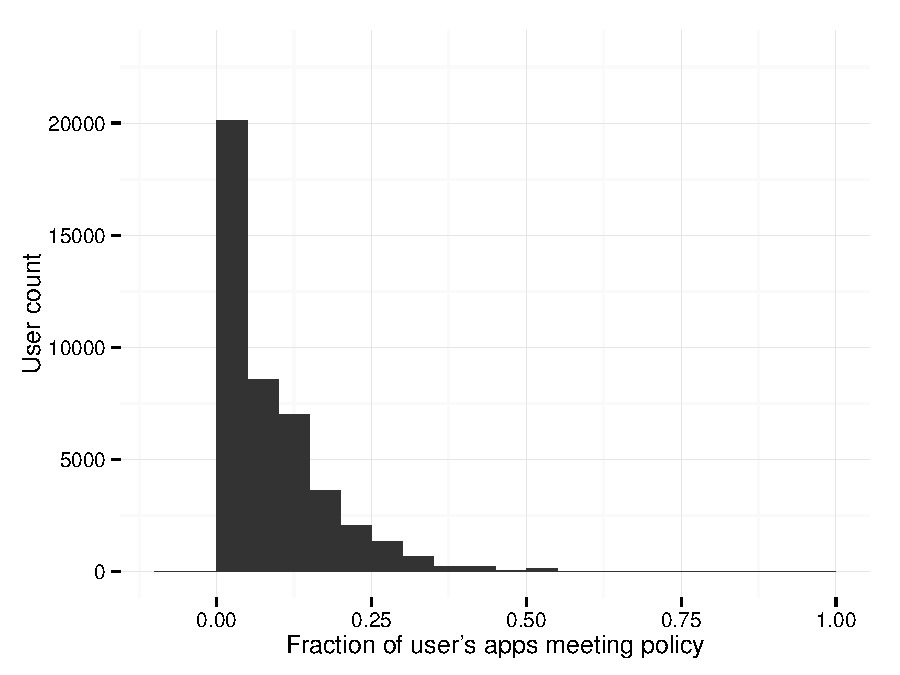
\includegraphics[width=0.5\linewidth]{figures/lin_a.pdf} 
  }
  \subfloat[Conservative policy]{%
    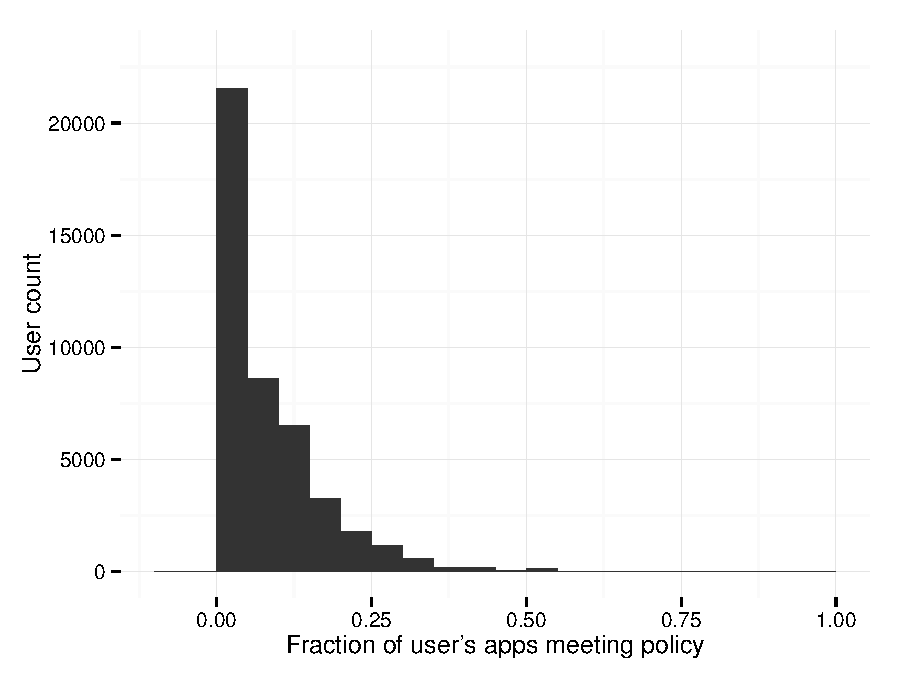
\includegraphics[width=0.5\linewidth]{figures/lin_c.pdf} 
  }\\
  \subfloat[Fencesitter policy]{%
    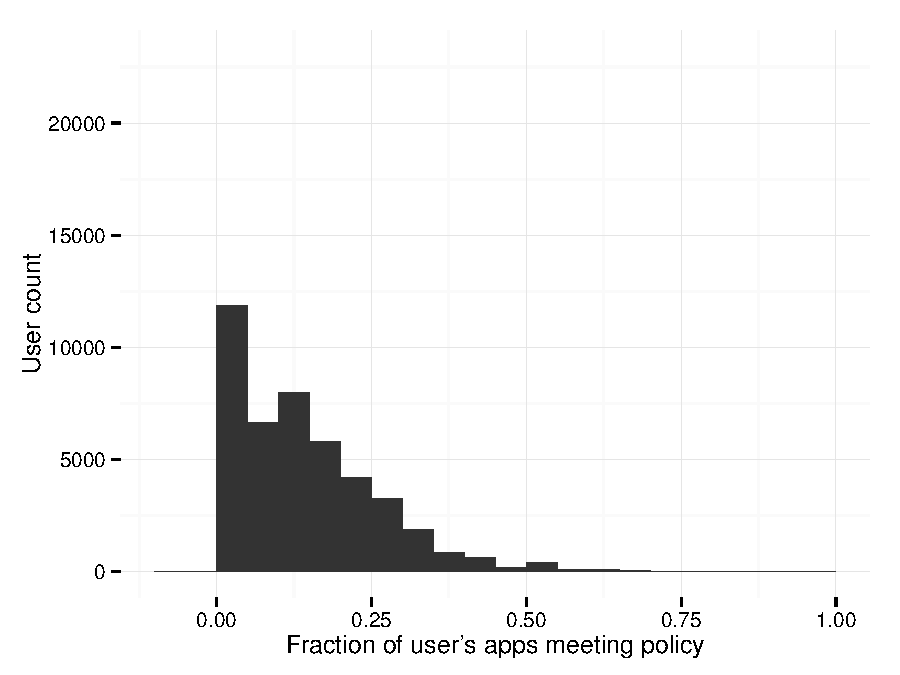
\includegraphics[width=0.5\linewidth]{figures/lin_f.pdf} 
  }
  \subfloat[Unconcerned policy]{%
    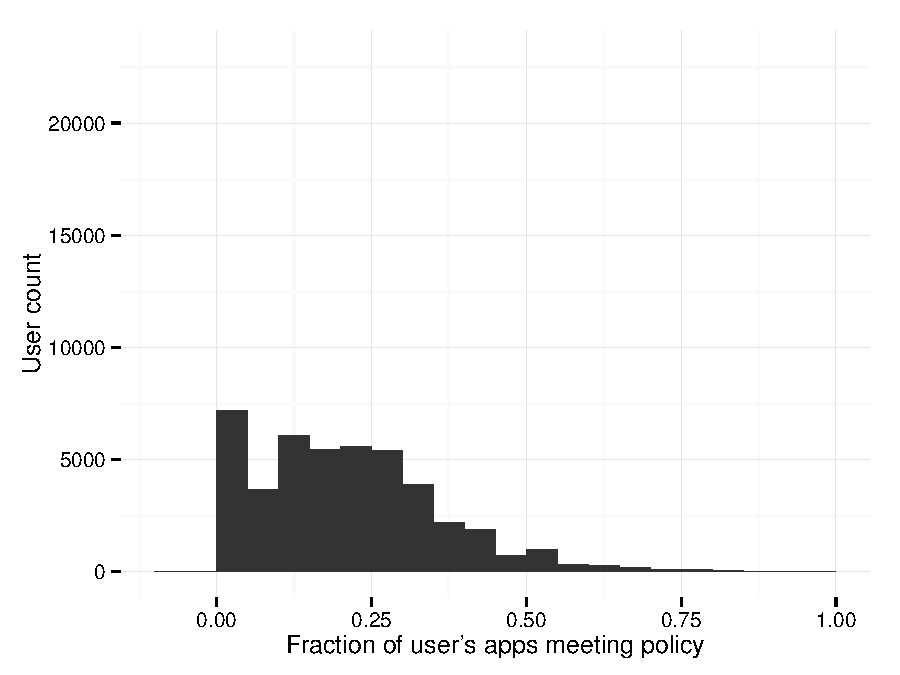
\includegraphics[width=0.5\linewidth]{figures/lin_u.pdf} 
  }\\
  \vspace{2em}
  \caption[Adoption of Lin~\etal~policies.]{Adoption of the four Lin~\etal~policies amongst users from the Carat dataset.  The vast majority of users do not appear to be following these policies most of the time.}
  \label{fig:lin_uptake_graphs}
\end{figure*}

The charts shown in \autoref{fig:lin_uptake_graphs} show that very few users seem to follow Lin~\etal's policies most of the time~\cite{hallett_apppal_2016}.  Even for the least onourus unconcerned policy most users did not seem to follow the policy most of the time.
This suggests that there is a disconnect between user's privacy preferences and their behavior (reminiscent of the \emph{privacy paradox}\footnote{The privacy paradox is that whilst people will say they are very concerned about their privacy, they do not alter their behaviour in order to protect it.  It was first noticed by psychologists looking at how people use social network; though has appeared in many other areas since.}); assuming the user population studied by Lin~\etal~was similar to the data in the Carat study.

A few users, however, did seem to be installing apps meeting these policies most of the time.
This suggests that while users may have privacy preferences the majority are not attempting to enforce them.
Policy enforcement tools, like AppPAL, can help users enforce their own policies which they cannot do easily using the current ad hoc, manual means available to them.

It is also interesting to discover when people install apps classified as malware.
McAfee classify malware into several categories, and provided us with a dataset of apps classified as malware and \acp{PUP}.
The \emph{malicious} and \emph{trojan} categories describe traditional malware.
Other categories classify \ac{PUP} such as aggressive adware.
Using AppPAL we can write policies to differentiate characterising users who allow dangerous apps and those who install poor quality ones.
\begin{lstlisting}
'user' says 'mcafee' can-say
  'malware' isKindOf(App).
'mcafee' says 'trojan' can-act-as 'malware'.
'mcafee' says 'pup' can-act-as 'malware'.
\end{lstlisting}
If a user is enforcing a privacy policy we might also expect them to install less malware.
We can check this by using AppPAL policies to measure the number of malwares each user had installed.

\begin{marginfigure}
  \centering
  \subfloat[Malware only]{%
    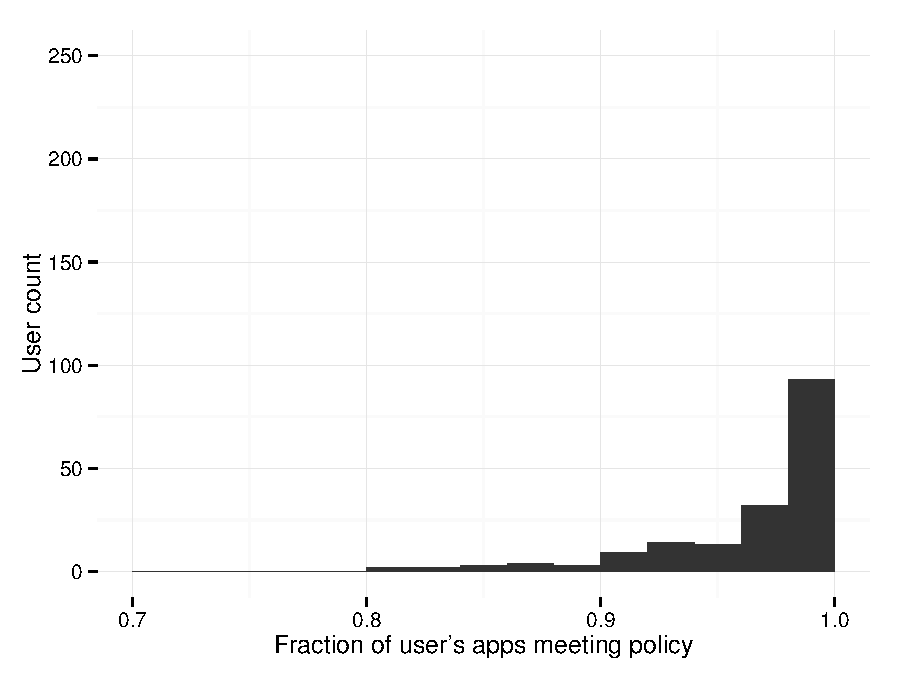
\includegraphics[width=\linewidth]{figures/malware_np.pdf}
  }\\
  \subfloat[Malware and PUPs]{%
    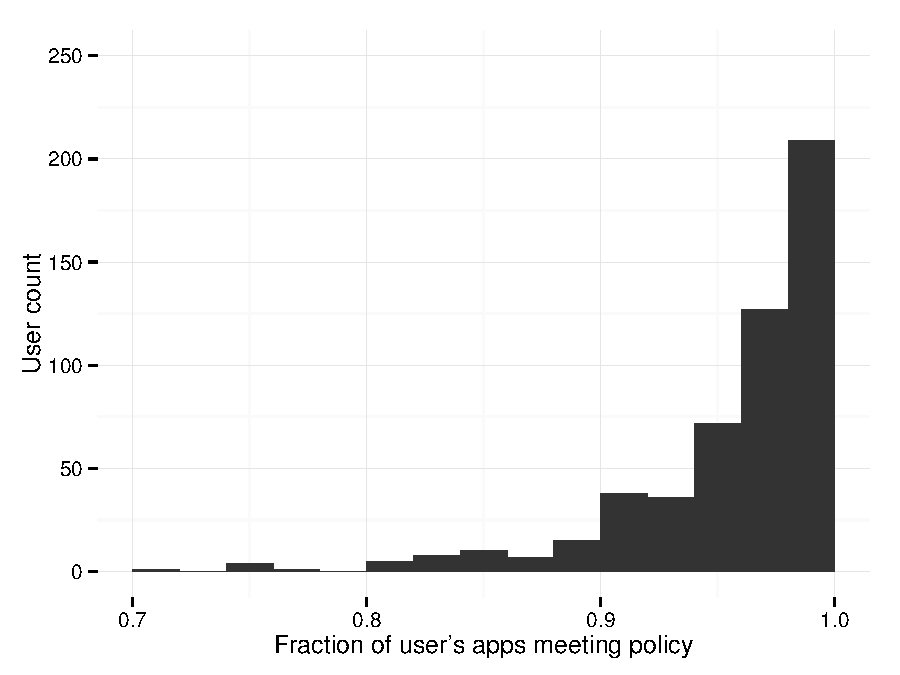
\includegraphics[width=\linewidth]{figures/malware_nm.pdf}
  }\\
  \caption{Malware installation numbers in the Carat dataset.}
  \label{fig:malware}
\end{marginfigure}
We found that 1\% of the users had a \ac{PUP} or malicious app installed.
Figure~\ref{fig:malware} shows that infection rates for \acp{PUP} and malware is low;
though a user is 3 times more likely to have a \ac{PUP} installed than malware.
It is interesting to compare a user's compliance to the Lin~\etal~policies with the amount of malware each had installed (Figure \autoref{fig:lin_malware_graphs}).
Users who were complying more than half the time with the conservative or advanced policies complied with the malware or \ac{PUP} policies fully.
This suggests that policy enforcement is worthwhile: users who do enforce policies about their apps experience less malware.
This could also be attributed to the users needing to be more selective about their apps in order to enforce their policy: a careful user is unlikely to install malware generally.

\begin{figure*}
  \centering
  \subfloat[Advanced policy and malware]{%
    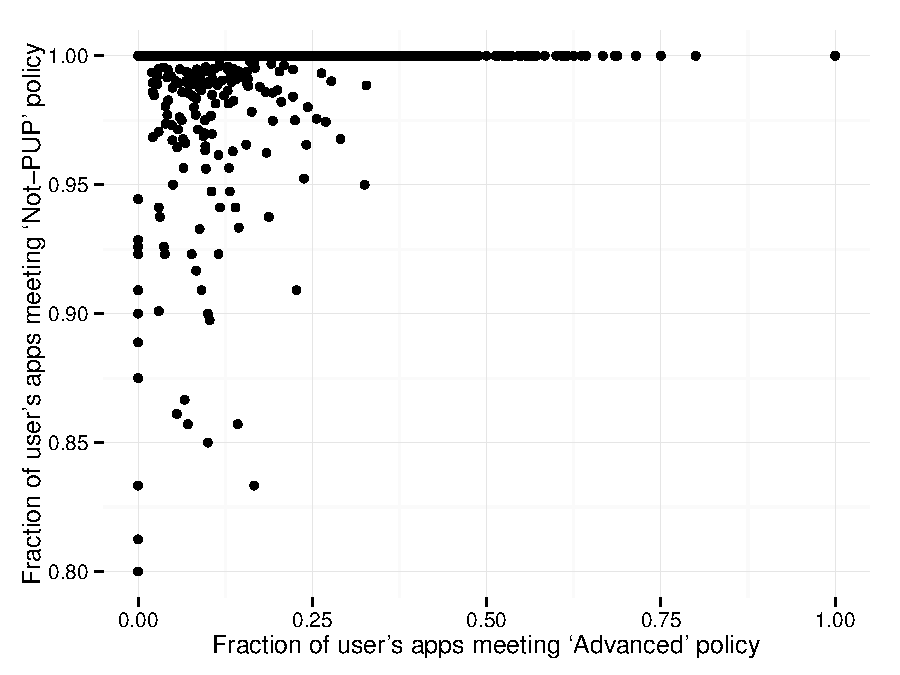
\includegraphics[width=0.5\linewidth]{figures/advanced-v-pup.pdf} 
  }
  \subfloat[Conservative policy and malware]{%
    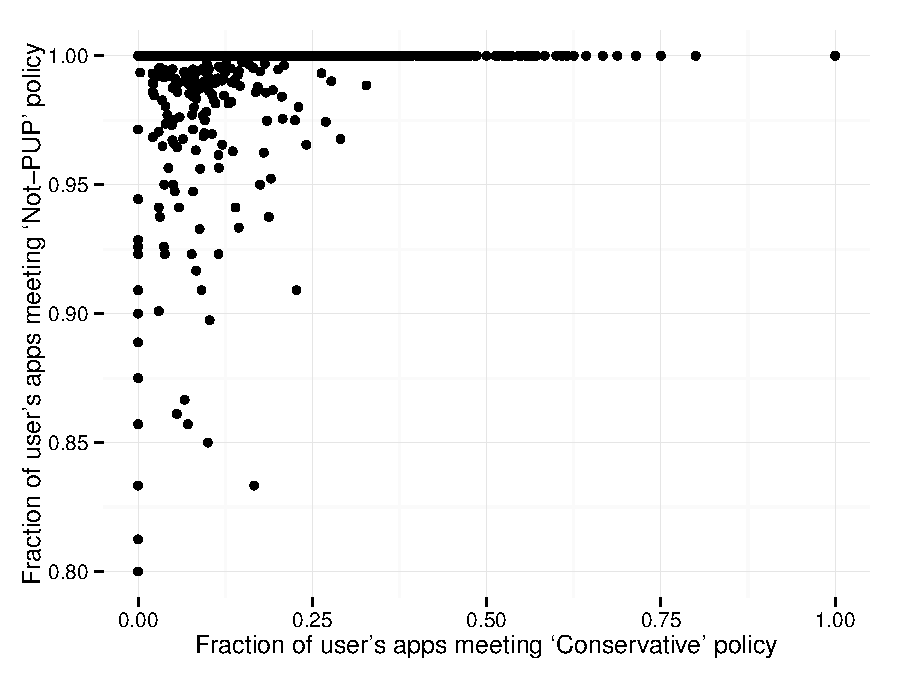
\includegraphics[width=0.5\linewidth]{figures/conservative-v-pup.pdf}
  }\\
  \subfloat[Fencesitter policy and malware]{%
    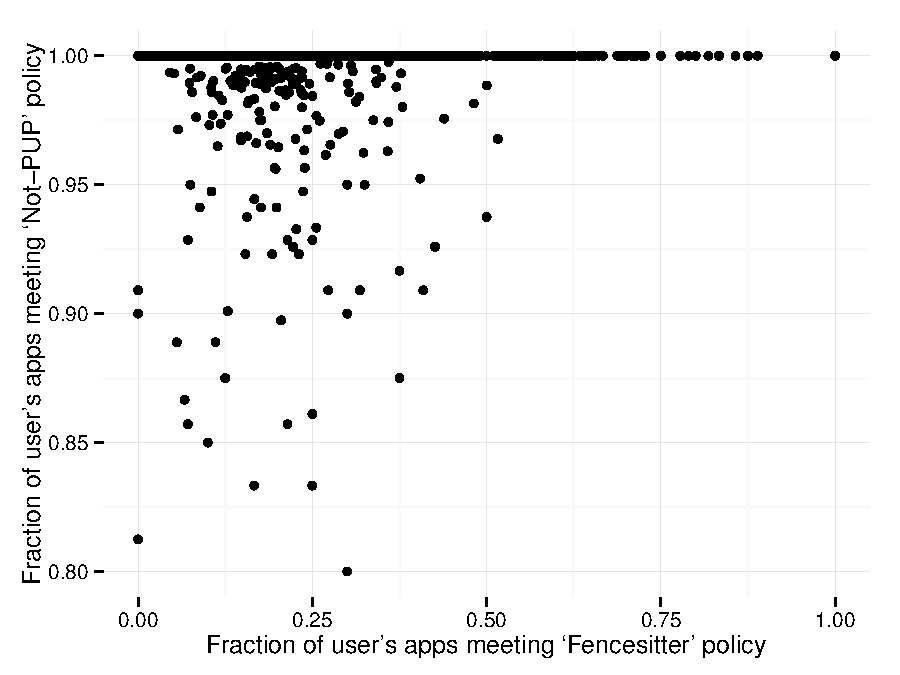
\includegraphics[width=0.5\linewidth]{figures/fencesitter-v-pup.pdf}
  }
  \subfloat[Unconcerned policy and malware]{%
    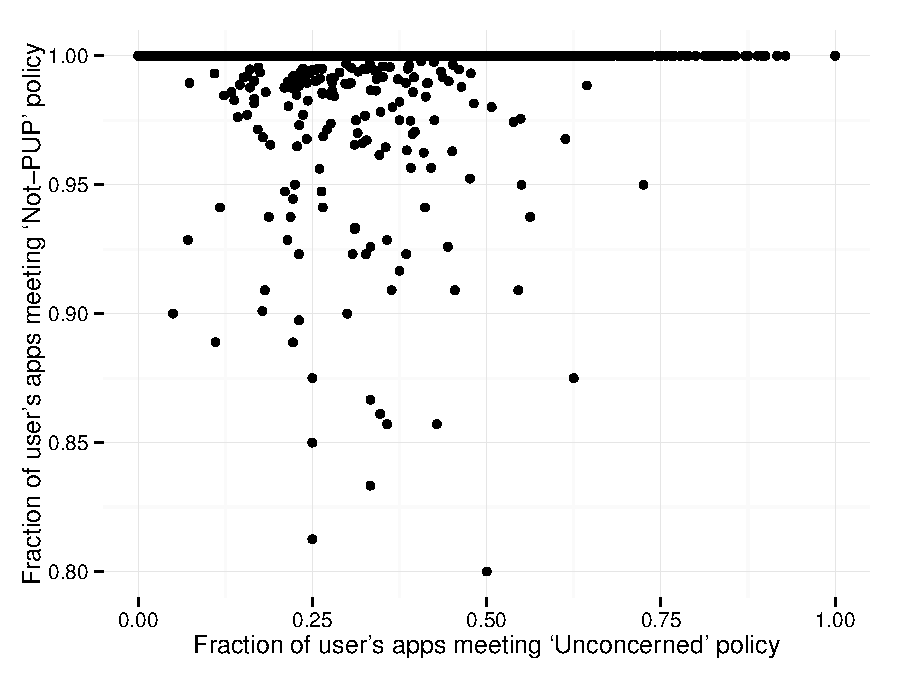
\includegraphics[width=0.5\linewidth]{figures/unconcerned-v-pup.pdf}
  }\\
  \vspace{2em}
  \caption[Plots of compliance with the Lin policies versus malware installation.]{Graphs plotting a users conformance with the Lin~\etal~policies against the amount of malware they had installed on their device.  Each dot represents a user.}
  \label{fig:lin_malware_graphs}
\end{figure*}


\section{An AppPAL Enhanced Store}

Using AppPAL we can describe user's preferences for apps, and we can describe
the differences between some of the stores.  A natural continuation of this is
to start to generate new app stores, based on a user's policy, that only sell
apps that a user might find acceptable.

Curated app stores are a similar idea, used inside companies to help employees
install apps for work that satisfy company policies (as will be expanded upon
in \autoref{chap:byod}).  With these corporate stores the apps are handselected
by IT staff.  Other stores, such as \emph{F-Droid}, effectively act as public
curated stores by only accepting apps that meet their requirements for an Open
Source licence.

\begin{figure}\centering
  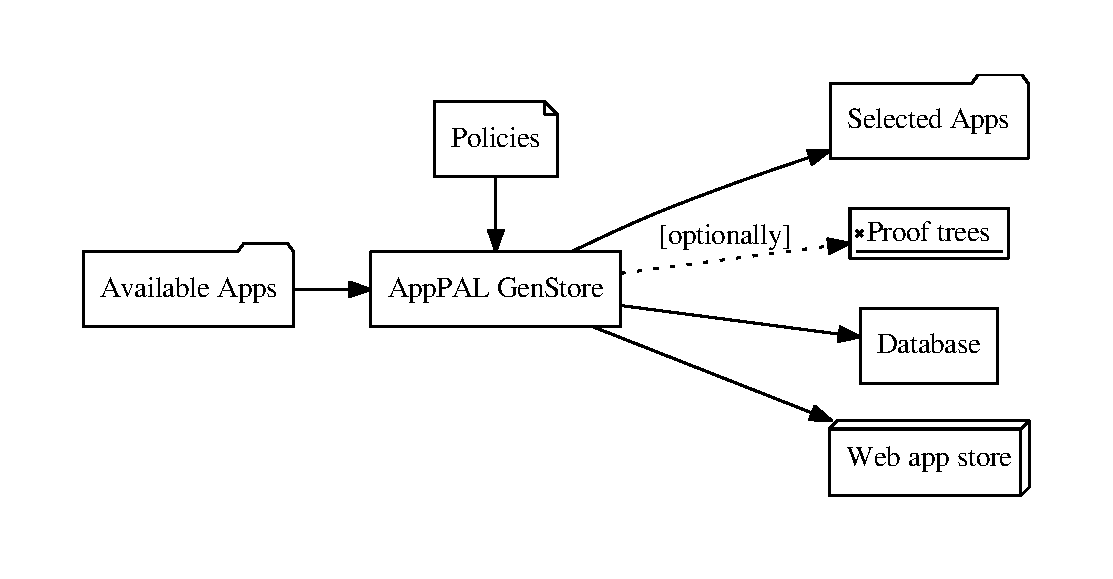
\includegraphics[width=\textwidth]{figures/genstore.pdf}
  \caption[AppPAL GenStore's architecture.]{AppPAL GenStore's architecture.  In go policies and apps, out come app stores.}
  \label{fig:genstore-architecture}
\end{figure}

AppPAL's \emph{GenStore} tool automates this process for Android app stores.  The architecture is shown in \autoref{gif:genstore-architecture}, though it can be summarised as:

\begin{enumerate}
\item The developer provides a pool of apps to GenStore. GenStore will select from amongst these apps to create the curated store.
\item The developer also provides a series of policy files. These should include rules to decide if an \emph{App isSellable}.  Optionally they can also describe predicates where \emph{App hasCategory(Category)} which will be used to organise the apps into categories in the store.
\item GenStore runs, and for every app checks whether it is \emph{sellable}.  Additionally it checks apps for each category (apps can belong to multiple categories), if defined.
  From this the GenStore builds a database (\autoref{fig:genstore-schema}) documenting which apps are avilable, their catagories and soem additional metadata.
\item A webapp is created from a template.  The default template uses the Sinatra framework to serve the store, but any framework could be used.  Alongside the webapp, the selected APK files are copied into a directory and a database is created storing information about the apps.
\end{enumerate}

Genstore is a prototype, but it lets developers explore how policies could be integrated into the Android ecosystem.
It shows an example of how AppPAL can be used to help make decisions, in this case about which apps make the cut for a store, automatically.
For a company seeking to enforce a policy about which apps are installable they could use it to offer their employees choice about apps, without having to remove the default store entirely.
If an AV vendor integrated their own checks into AppPAL then they could trivially create a \emph{safe} app store where all apps have been demonstrably vetted by their software and engineers.

\begin{figure}\centering
  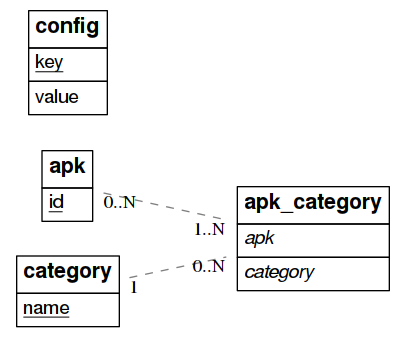
\includegraphics[width=0.4\textwidth]{figures/genstore-schema.png}
  \caption{GenStore database schema.}
  \label{fig:genstore-schema}
\end{figure}

\begin{figure}\centering
  \framebox[\textwidth]{TODO: ADD SCREENSHOT WHEN I FIX THE BUGS\vspace{3in}}
  \caption{Screenshot of a generated store.}
  \label{fig:genstore-screenshot}
\end{figure}

\end{document}


%%% Local Variables:
%%% mode: latex
%%% TeX-master: "../../thesis"
%%% End
